% Created 2020-07-21 mar 12:10
% Intended LaTeX compiler: pdflatex
\documentclass[presentation,aspectratio=1610]{beamer}
\usepackage[utf8]{inputenc}
\usepackage[T1]{fontenc}
\usepackage{graphicx}
\usepackage{grffile}
\usepackage{longtable}
\usepackage{wrapfig}
\usepackage{rotating}
\usepackage[normalem]{ulem}
\usepackage{amsmath}
\usepackage{textcomp}
\usepackage{amssymb}
\usepackage{capt-of}
\usepackage{hyperref}
\usepackage{khpreamble, euscript}
\DeclareMathOperator{\atantwo}{atan2}
\newcommand*{\ctrb}{\EuScript{C}}
\newcommand*{\obsv}{\EuScript{O}}
\usetheme{default}
\author{Kjartan Halvorsen}
\date{\today}
\title{Control computarizado - Modelos en espacio de estados}
\hypersetup{
 pdfauthor={Kjartan Halvorsen},
 pdftitle={Control computarizado - Modelos en espacio de estados},
 pdfkeywords={},
 pdfsubject={},
 pdfcreator={Emacs 26.3 (Org mode 9.3.6)}, 
 pdflang={English}}
\begin{document}

\maketitle

\section{Intro}
\label{sec:org98e0d20}
\begin{frame}[label={sec:orgaf1f3ac}]{Ejemplo - El modulo lunar de Apollo}
\begin{center}
\includegraphics[width=\linewidth]{fig-apollo}
\end{center}
\end{frame}
\begin{frame}[label={sec:orge6377ae}]{Ejemplo - El modulo lunar de Apollo}
\begin{center}
\includegraphics[width=0.8\linewidth]{fig-apollo}
\end{center}
\alert{Actividad} ¿Cuál es la función de transferencia del sistema?
\[1: \; G(s) = \frac{k_1 k_2}{s^2}\qquad 2: \; G(s) = \frac{k_1 k_2}{s(s^2 + 1)} \qquad 3: \; G(s) = \frac{k_1 k_2}{s^3}\]
\end{frame}

\begin{frame}[label={sec:orgdca7e5d}]{Ejemplo - El modulo lunar de Apollo}
\begin{center}
\includegraphics[width=0.8\linewidth]{fig-apollo}
\end{center}
\alert{Actividad} ¿Que sensores relevantes se puede usar para el control?
\end{frame}

\begin{frame}[label={sec:orgd1eec8a}]{Ejemplo - El modulo lunar de Apollo}
\begin{center}
\includegraphics[width=0.7\linewidth]{fig-apollo}
\end{center}

Variables del estado: \(x = \begin{bmatrix} x_1 & x_2 & x_3 \end{bmatrix}^T = \begin{bmatrix} \dot{\theta} & \theta & \dot{z} \end{bmatrix}^T\). Con dinamica
\[ \begin{cases} \dot{x}_1 =  \ddot{\theta} = k_1 u\\ \dot{x}_2 = \dot{\theta} = x_1\\ \dot{x}_3 = \ddot{z} = k_2\theta = k_2x_2 \end{cases} \]
\end{frame}

\begin{frame}[label={sec:orgddf4b9f}]{Ejemplo - El modulo lunar de Apollo}
Variables del estado: \(x = \begin{bmatrix} x_1 & x_2 & x_3 \end{bmatrix}^T = \begin{bmatrix} \dot{\theta} & \theta & \dot{z} \end{bmatrix}^T\). Con dinamica
\[ \begin{cases} \dot{x}_1 =  \ddot{\theta} = k_1 u\\ \dot{x}_2 = \dot{\theta} = x_1\\ \dot{x}_3 = \ddot{z} = k_2\theta = k_2x_2 \end{cases} \]

\alert{Actividad} Llena los matrices y vectores en el modelo de espacio de estados

\[ \dot{x} = \begin{bmatrix} \dot{x}_1\\\dot{x}_2\\\dot{x}_3\end{bmatrix} = \underbrace{\begin{bmatrix} \quad & \quad &\quad \\\quad & \quad& \quad\\ \quad& \quad &\quad \end{bmatrix}}_{A} \begin{bmatrix} x_1\\x_2\\x_3\end{bmatrix} + \underbrace{\begin{bmatrix} \quad \\ \quad \\\quad  \end{bmatrix}}_{B} u \]
\end{frame}


\begin{frame}[label={sec:org67996e0}]{Discretización}
Solución general de un sistema lineal en espacio de estados 
\begin{align*}
x(t_k+\tau)& = \mathrm{e}^{A(\tau)} x(t_k) + \int_{0}^\tau \mathrm{e}^{As} B u\big((t_k+\tau)-s) ds
\end{align*}

\begin{center}
  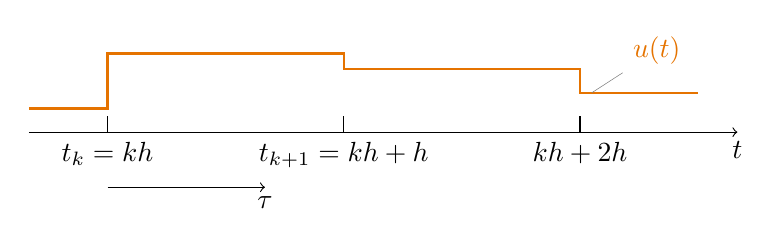
\begin{tikzpicture}
    \draw[->] (-3,0) -- (6,0) node[below] {$t$};
    \draw (-2, 0.2) -- ( -2, 0) node[below] {$t_k=kh$};
    \draw (1, 0.2) -- ( 1, 0) node[below] {$t_{k+1}=kh+h$};
    \draw (4, 0.2) -- ( 4, 0) node[below] {$kh+2h$};
    \draw[thick, orange!90!black] (-3,0.3) -- (-2, 0.3) -- (-2,1) -- (1, 1) -- (1,0.8) -- (4, 0.8) --(4, 0.5) --(5.5, 0.5) node[pos=0.1, coordinate, pin=30:{$u(t)$}] {} ; 
    \draw[->] (-2, -0.7) -- (0, -0.7) node[below] {$\tau$};
  \end{tikzpicture}
\end{center}

 \begin{align*}
  x(kh+h) &= \mathrm{e}^{Ah} x(kh) + \int_{0}^{h} \mathrm{e}^{As} B u(kh+h-s) ds\\
   &= \underbrace{\mathrm{e}^{Ah}}_{\Phi(h)} x(kh) + \underbrace{\left(\int_{0}^h \mathrm{e}^{As} B ds \right)}_{\Gamma(h)} u(kh)
\end{align*}
\end{frame}

\begin{frame}[label={sec:orgd0597b2}]{Discretización - La exponencial de una matriz}
Matriz \(A\) cuadrada. Variable \(t\) escalar.
\[ \mathrm{e}^{At} = 1 + At + \frac{t^2}{2!}A^2 + \frac{t^3}{3!} A^3 + \cdots\]
Transformada de Laplace:
\[ \laplace{\mathrm{e}^{At}} = (sI - A)^{-1}\]
\end{frame}


\begin{frame}[label={sec:orgd4c9dc3}]{Discretización - ejemplo}
 \begin{align*}
  x(kh+h) &= \mathrm{e}^{Ah} x(kh) + \int_{0}^{h} \mathrm{e}^{As} B u(kh+h-s) ds\\
   &= \underbrace{\mathrm{e}^{Ah}}_{\Phi(h)} x(kh) + \underbrace{\left(\int_{0}^h \mathrm{e}^{As} B ds \right)}_{\Gamma(h)} u(kh)
\end{align*}
\[ A = \begin{bmatrix} 0 & 0 & 0\\1 & 0 & 0\\0 & k_2 & 0\end{bmatrix}, \quad A^2 = \begin{bmatrix} 0 & 0 & 0\\1 & 0 & 0\\0 & k_2 & 0\end{bmatrix}\begin{bmatrix} 0 & 0 & 0\\1 & 0 & 0\\0 & k_2 & 0\end{bmatrix}= \begin{bmatrix} 0 & 0 & 0\\0 & 0 & 0\\k_2 & 0  & 0\end{bmatrix}, \quad A^3 = 0\]
Entonces,
\begin{align*}
 \Phi(h) &= \mathrm{e}^{Ah} = 1 + Ah + A^2 h^2/2  + \cdots \\
 &= \begin{bmatrix} 1 & 0 & 0\\0 & 1 & 0\\0 & 0 & 1\end{bmatrix} + \begin{bmatrix} 0 & 0 & 0\\1 & 0 & 0\\0 & k_2 & 0\end{bmatrix}h + \begin{bmatrix} 0 & 0 & 0\\0 & 0 & 0\\k_2 & 0 & 0\end{bmatrix}\frac{h^ 2}{2}= \begin{bmatrix} 1 & 0 & 0\\h & 1 & 0\\\frac{h^2k_2}{2} & hk_2 & 1\end{bmatrix}
 \end{align*}
\end{frame}

\begin{frame}[label={sec:orgf46e687}]{Discretización - ejemplo}
 \begin{align*}
  x(kh+h) &= \mathrm{e}^{Ah} x(kh) + \int_{0}^{h} \mathrm{e}^{As} B u(kh+h-s) ds\\
   &= \underbrace{\mathrm{e}^{Ah}}_{\Phi(h)} x(kh) + \underbrace{\left(\int_{0}^h \mathrm{e}^{As} B ds \right)}_{\Gamma(h)} u(kh)
\end{align*}
\[\mathrm{e}^{As}B &=  \begin{bmatrix} 1 & 0 & 0\\h & 1 & 0\\\frac{s^2k_2}{2} & sk_2 & 1\end{bmatrix} \begin{bmatrix} k_1\\0\\0 \end{bmatrix} = k_1 \begin{bmatrix} 1\\s\\\frac{k_2s^2}{2} \end{bmatrix}
  \]
\begin{align*}
\Gamma (h) &= \int_0^h \mathrm{e}^{As}B ds = k_1 \int_0^h \begin{bmatrix} 1\\s\\\frac{k_2s^2}{2} \end{bmatrix}ds = k_1\begin{bmatrix} h\\ \frac{h^2}{2} \\ \frac{k_2 h^3}{6} \end{bmatrix} 
\end{align*}
\end{frame}

\begin{frame}[label={sec:orgb26a856}]{Discretización - ejemplo}
 \begin{align*}
  x(kh+h) &= \mathrm{e}^{Ah} x(kh) + \int_{0}^{h} \mathrm{e}^{As} B u(kh+h-s) ds\\
   &= \underbrace{\mathrm{e}^{Ah}}_{\Phi(h)} x(kh) + \underbrace{\left(\int_{0}^h \mathrm{e}^{As} B ds \right)}_{\Gamma(h)} u(kh)\\
   &= \begin{bmatrix} 1 & 0 & 0\\h & 1 & 0\\\frac{h^2k_2}{2} & hk_2 & 1\end{bmatrix} x(kh) + k_1 \begin{bmatrix} h\\ \frac{h^2}{2} \\ \frac{k_2 h^3}{6} \end{bmatrix} u(kh)
\end{align*}
\end{frame}



\section{Stability, controllability, observability}
\label{sec:org2434a51}
\begin{frame}[label={sec:org41fe909}]{Goal of today's lecture}
\begin{itemize}
\item Understand state feedback design
\end{itemize}
\end{frame}

\section{State space models repetition}
\label{sec:org030c453}

\begin{frame}[label={sec:orgac3bf38}]{Stability}
A system 
\begin{equation*}
x(k+1)=\Phi x(k), \ \ x(0)=x_0
\end{equation*}
is \emph{asymptotically stable}  if  \(\underset{t\to\infty}{\lim}x(kh)=0\) for all  \(x_0\in\Bbb{R}^n\).\\

A system is asymptotically stable if and only if \alert{all eigenvalues of \(\Phi\) are inside the unit circle.}
\end{frame}

\begin{frame}[label={sec:orga5ee6ab}]{Reachability (controllability)}
Reachability is the answer to the question "Can we by choosing a suitable input sequence \(u(k),\; k=0,1,2,\ldots,n-1\) reach any point in the state space?"

Consider
\[ x(k+1) = \Phi x(k) + \Gamma u(k). \]
With initial state \(x(0)\) given. The solution at time \(n\) where \(n\) is the order of the system is
\begin{equation}
\begin{split}
x(n) &= \Phi^nx(0) + \Phi^{n-1}\Gamma u(0) + \cdots + \Gamma u(n-1)\\
     &= \Phi^nx(0) + W_c U, 
\end{split}
\end{equation}
where
\begin{align*}
W_c &= \bbm \Gamma & \Phi\Gamma & \cdots & \Phi^{n-1}\Gamma\ebm\\
U &= \bbm u(n-1) & u(n-2) & \cdots & u(0) \ebm\transp
\end{align*}
\end{frame}

\begin{frame}[label={sec:org458121a}]{Reachability (controllability), contd}
To find the input sequence that takes the state to \(x(n) = x_d\) we solve the equation
\[ x_d = \Phi^nx(0) + W_cU\]
for \(U\). 

\[ U = W_c\inv \left(x_d - \Phi^nx(0)\right) \]

This requires the matrix \(W_x\) to be \alert{invertible}. This gives Theorem 3.7 in Å\&W:

THEOREM 3.7 REACHABILITY The state space system above is reachable if and only if the matrix \(W_c\) has rank \(n\). 

This is equivalent to 
\[ \det W_c \neq 0.\]
\end{frame}

\section{State feedback}
\label{sec:org171c6af}
\begin{frame}[label={sec:org4147ce9}]{State feedback}
Have state space model
 \begin{equation}
 \begin{split}
  x(k+1) &= \Phi x(k) + \Gamma u(k)\\
  y(k) &= C x(k)
 \end{split}
 \label{eq:ssmodel}
\end{equation}
and measurements (or estimates) of the state vector \(x(k)\). 

\alert{Linear state feedback} is the control law
\begin{equation*}
\begin{split}
 u(k) &= f\big((x(k), u_c(k)\big) = -l_1x_1(k) - l_2x_2(k) - \cdots - l_n x_n(k) + mu_c(k)\\
      &= -Lx(k) + mu_c(k), 
\end{split}
\end{equation*}
where \[ L = \bbm l_1 & l_2 & \cdots & l_n \ebm. \]

Insert the control law into the state space model \eqref{eq:ssmodel} to get
\end{frame}
\begin{frame}[label={sec:org503fa75}]{State feedback}
Have state space model
 \begin{equation}
 \begin{split}
  x(k+1) &= \Phi x(k) + \Gamma u(k)\\
  y(k) &= C x(k)
 \end{split}
 \label{eq:ssmodel}
\end{equation}
and measurements (or estimates) of the state vector \(x(k)\). 

\alert{Linear state feedback} is the control law
\[ u(k) = -l_1x_1(k)  -l_2x_2(k) - \cdots - l_n x_n(k) + mu_c(k)= -Lx(k) + mu_c(k), \]
where \[ L = \bbm l_1 & l_2 & \cdots & l_n \ebm. \]

Insert the control law into the state space model \eqref{eq:ssmodel} to get
 \begin{equation}
 \begin{split}
  x(k+1) &= \left(\Phi -\Gamma L \right) x(k) + m\Gamma u_c(k)\\
  y(k) &= C x(k)
 \end{split}
 \label{eq:closedloop}
\end{equation}
\end{frame}

\begin{frame}[label={sec:org9569d41}]{Pole placement by state feedback}
Assume the desired performance of the control system is given as a set of desired closed loop poles \(p_1, p_2, \ldots, p_n\), corresponding to the desired characteristic polynomial
\begin{equation}
a_c(z) = (z-p_1)(z-p_2)\cdots(z-p_n) = z^n + \alpha_1 z^{n-1} + \cdots \alpha_n.
\label{eq:desiredpoles}
\end{equation}

With state feedback we get the the closed-loop system
 \begin{equation}
 \begin{split}
  x(k+1) &= \left(\Phi -\Gamma L \right) x(k) + m\Gamma u_c(k)\\
  y(k) &= C x(k)
 \end{split}
 \label{eq:closedloop}
\end{equation}
with characteristic equation
\begin{equation}
\det\left(zI - (\Phi - \Gamma L)\right) = z^n + \beta_1(l_1,\ldots,l_n) z^{n-1} + \cdots \beta_n(l_1, \ldots, l_n).
\label{eq:poles}
\end{equation}

Equate the coefficients in \eqref{eq:desiredpoles} and \eqref{eq:poles} to get the system of equations
\begin{equation*}
\begin{split}
\beta_1(l_1, \ldots, l_n) &= \alpha_1\\
\beta_2(l_1, \ldots, l_n) &= \alpha_2\\
&\vdots\\
\beta_n(l_1, \ldots, l_n) &= \alpha_n
\end{split}
\label{eq:coeffs}
\end{equation*}
\end{frame}

\begin{frame}[label={sec:orgb5ad2be}]{Pole placement by state feedback, contd.}
The system of equations
\begin{equation*}
\begin{split}
\beta_1(l_1, \ldots, l_n) &= \alpha_1\\
\beta_2(l_1, \ldots, l_n) &= \alpha_2\\
&\vdots\\
\beta_n(l_1, \ldots, l_n) &= \alpha_n
\end{split}
\label{eq:coeffs}
\end{equation*}
is always linear in the unknown controller parameters, so it can be written
\begin{equation*}
A L\transp = \alpha,
\end{equation*}
Where \(\alpha\transp = \bbm \alpha_1 & \alpha_2 & \cdots & \alpha_n \ebm.\)
\end{frame}

\begin{frame}[label={sec:org7ccbf2d}]{Pole placement and reacability}
It can be shown that the controllability matrix \(W_c\) is a factor of the matrix \(A\)
\[ A = \bar{A} W_c. \] Hence, in general the system of equations
\begin{equation}
\bar{A}W_c L\transp = \alpha
\label{eq:poleplace}
\end{equation}
has a solution only if \(W_c\) is invertible, i.e. the system is \emph{reachable}.

Note that equation \eqref{eq:poleplace} can still have a solution for unreachable systems if \alert{\(\alpha\) is in the \emph{column space} of \(A\)}, i.e. \(\alpha\) can be written
\[ \alpha = b_1 A_{:,1} + b_2A_{:,2} + \cdots + b_mA_{:,m}, \; m < n \]
\end{frame}
\end{document}